\documentclass{article}
\usepackage{graphicx}
\usepackage{tabto}
\usepackage{amssymb}
\usepackage[a4paper, total={6in, 8in}]{geometry}

\begin{document}

\begin{titlepage}
    \centering
    \vfill
    {\bfseries\Large STMF32 Discovery Board: Sensor Data Acquisition and Display}    
    \vskip2cm
    
\includegraphics[width=4cm]{mcgill_logo.png}
    
    \vskip2cm
    \large\textbf{ECSE 426} \\
    \large\textbf{Lab 2 - Report} \\
	\vskip0.2cm

    \vskip1.3cm
    \textbf{Group 20}
    \vskip0.2cm
      Habib Ahmed \\
      260464679 \\
    \vskip0.4cm
      Aditya Saha \\
      260453165 \\
    \vskip0.5cm
	McGill University \\
    February, 2016
    \vfill
\end{titlepage}
\newpage

\tableofcontents
\newpage

\section{Abstract}
One of the most commonly used applications of embedded microprocessor systems is to acquire data and perform conditioning of signals by using application-specific sensors. Obtaining temperature readings is one such example [1]. The purpose of this experiment was to use the onboard temperature sensor of the STM32F4-Discovery board, along with a 7-segment display to obtain and display the real-time temperature of the processor. Signal conditioning was also necessary given its noisy nature. Building the external circuitry of the 7-segment display and interfacing it through the digital I/O pins, in order to display the numeric values of the temperature, was also required.  

\section{Problem Statement}
\begin{itemize}
\item \textbf{Setting up the temperature sensor and ADC:} The primary objective for our lab was to utilize the onboard temperature sensor to measure the temperature of the processor. The purpose of the analog to digital to converter was to make use of the raw analog data from the sensor, the voltage in this case, and obtain the correct temperature reading (digitally). This required setting up the correct channel for the ADC as well as write the equation for converting the raw value. The temperature readings would be acquired at a frequency of 100Hz.
\item \textbf{Setting up the sampling frequency:} The second objective was to use the SysTick timer to set up the sampling frequency for the data of 100Hz.
\item \textbf{Signal filtering:} The third objective was to remove the noise from the raw data so that the temperature readings are more accurate. This was to be done by using the Kalman Filter that was implemented in lab 1. An additional goal was to determine the initial conditions that produced the best temperature readings.
\item \textbf{Making sense of data:} The voltage readings needed to be converted to temperature in degrees Celsius.
\item \textbf{Temperature display:} The calculated temperature value is then displayed on a 7-segment display.
\item \textbf{Overheating alarm:} The implementation of an overheating alarm, LED signals in this case, is required when the temperature of the processor exceeds a certain value. The temperature threshold for this was determined by us.
\end{itemize}

\section{Theory and Hypothesis}
While the problem statement was mostly straightforward, special consideration had to be taken while designing the temperature display and elimination of noisy data by signal processing. The issue with the display was that it was a common-cathode type display and a multiplexing circuit had to be implemented to make each segment light up individually [2]. To accomplish this, the resistors and transistors provided would have to be used to build an external circuit that would allow the switching on and off of the different segments. The time duration for which each individual segment should be lit up was also predetermined.\\

\noindent To eliminate noise, the Kalman Filter, which is  a  state-based  adaptive  estimator  of  a  physical  process  that  is  known  to  be optimal with respect to the estimation error when the noise is Gaussian and the system is linear, from Lab 1 was put to use [3]. This filter is best put to use where continuous sampling is required since it uses an interative filtering method. The noisy voltage readings were to be passed onto the filter before calculating the temperature. The mathematical equation for the filter is given below: \\

\[ X_k = K_kZ_k + (1 - K_k) X_{k-1} \]
%\[ a_1^2 + a_2^2 = a_3^2 \]

\noindent Here, $X_k$ represents the current estimation of the temperature, $K_k$ represents the Kalman Gain, $Z_k$ represents the measured value of the temperature and $X_{k-1}$ represents the previous estimate of the temperature. \\

\noindent Unlike Lab 1 however, an additional task for this lab was to choose the parameters that would output the best results with the Kalman Filter. This has been discussed in more detail in the Testing and Observations section. \\

\section{Implementation}
\subsection{Configuring ADC and the Sensor}

Implementation of ADC involves first initializing the ADC configuration structures to enable the ADC peripherals and power for the bus APB2 that interfaces with the ADC1 peripheral. The embedded temperature sensor is internally connected to channel 16. The ADC features two clock schemes: ADCCLK is the clock for the analog circuitry that is common across all ADC peripherals – this is the clock of interest for this experiment. This clock is generated from the APB2 bus clock that is divided by a programmable pre-scaler, enabling the ADC peripheral to work at configurable frequencies. According to specification, the APB2 clock is set at 84 MHz, however the ADC peripherals supports maximum clock frequency of 36 MHz, hence ADC\_CLOCK\_SYNC\_PCLK\_DIV4 is specified to provide an operating frequency of 84 / 2 = 21 MHz. The resolution bits for the output data has been set to 12 bits in the data register – greater resolution translates to slower conversion, however for a system engaging only the temperature sensor, faster conversion rate is less crucial. Continuous conversion mode has been also been enabled instead of single-burst conversion, hence allowing continuous polling for data once conversion has completed (as evidenced by setting end-of-conversion flag). Since the embedded temperature sensor is the only peripheral of interest for this experiment, scan conversion mode has been disabled to avoid polling of multiple channels. Reader may reference system\_config.h and system\_config.c files to complement the above discussion. 

\subsection{Configuring Sampling Frequency}
\noindent The sampling frequency was setup by using ARM’s inherent HAL\_SYSTICK\_Config() method, which takes in frequency parameter based on the system’s core clock and the desired frequency to be configured. The system’s core clock operates at 168 MHz and the SysTick frequency provided in the specification is 100 Hz. Interrupt handler has also been defined by setting ticks parameter to 1. This gets checked in every iteration of the main loop before polling for end-of-conversion flag of ADC peripheral. The main.c and stm32f4xx\_it.c source files may be referred to for further implementation details. \\

\noindent The routines HAL\_ADC\_Start and HAL\_ADC\_PollForConversion starts the analog-to-digital conversion, and starts polling for end-of-conversion flag setting. After completion of digitizing each measurements the routine HAL\_ADC\_GetValue is called to extract the output value and reset the flag. Since ADC peripheral has been configured as continuous conversion mode, repeated start and stop of the sensor has been avoided.

\subsection{Signal Filtering}
The raw readings acquired from the ADC peripheral is very noisy and less representative of actual changes in the physical medium. In order to streamline and smoothen the digital signal a Kalman filter has been used. Kalman filter is a state-based adaptive estimator that is more efficient than fixed linear filters [3]. The adaption is performed by a sequence of discrete operations whereby the filter parameters change based on the value observed in the physical medium and the current state of the filter. The difference value between the estimated output and the actual input has the statistical properties of white noise – a feature that has been leveraged during system testing and analysis phase.\\

\noindent Two routines are crucial to the implementation of Kalman filter – notably the Reset() routine that configures the initial state parameters, and the Kalmanfilter\_C() that recursively updates the state parameters following the input values. This routine takes a double-valued input which is the digitized output from the ADC peripheral, pointer to a double that stores the processed output of the filter and a pointer to the Kalman state structure that updates parameters. The function also checks for unbounded output value and returns 1 if the value is NaN, and 0 otherwise. A pseudocode for the Kalman filter structure and the calling routines have been included in the Appendix for ease of reference. Reader may refer to the Testing and Observations section that discusses how the initial values of the Kalman state has been decided and the filter calibrated.

\subsection{Data Interpretation}
The output of the Kalman filter maybe treated directly using mathematical equation to extract the corresponding temperature value in degrees Celsius. The reference manual and the datasheet has been extensively reference in this regards to extract the following equation [5] [6]:\\

\[temperature = \frac{\frac{output * 3000}{4096} - V_{25}}{average\_slope} + 25\]

\noindent Details of parameters in the equation are as follows:
\begin{itemize}
\item output = output value of the Kalman filter (a double)
\item $V_{25}$ = 760 mV
\item average\_slope = 2.5
\end{itemize}

\subsection{Temperature Display}
	In order to display the temperature readings a 7-segment display has been integrated in the system. The 7-segment display interfaces with the GPIO port on the microprocessor board to set the individual segments as high or low. An external circuit has been assembled following the guidelines set forth in the specification – the circuit follows multiplexing design that conservatively uses the segment display pins for select lines and individual digit display.\\

\noindent The display implementation first involves initializing the GPIO configuration structures to enable the GPIO peripherals, and power for the bus AHB1 that interfaces with the peripherals. Since GPIO ports are only employed to set the display segments in this experiment, the ports have been configured as push-pull output without pull-up or pull-down activation. 3 GPIO ports have been configured in the final system design – 3 pins on PORTA for the display select lines,  8 pins on PORTE to set the unit segments to display digits and decimal point, and 4 pins on PORTD to toggle alarm LEDs (to be discussed in next section). The crux of the display logic is the Display() routine that lays out the required pin write configurations for the select lines (to choose digit display position – from most to least significant) and the digit display (between 0-9 and decimal point). Reader may consult the 7seg\_display.c source file for implementation details. The logic for display of unit digit employs case-switch structure to check which digit should be displayed and which corresponding segments should be set to accomplish the display. The datasheet has been referred to find out I/O pins available to be used. Caution has been exercised to not address the restricted I/O pins that are reserved for special debugging purposes.\\

\noindent The main.c source file refers to the Display() routine to incrementally display the digits that correspond to the interpreted temperature value (discussed in the previous section). However, prior to calling the Display() routine the individual digits must be extracted from the conversion value (a double). A simple iterative logic has been employed to accomplish this goal, a pseudocode has been included in the appendix for ease of reference for the readers. \\

\noindent As stated in specification, the system has been configured to sample temperature measurements at 100 Hz [1]. However, this is beyond visually perceivable by the human eye. Besides an efficient implementation has been sought out that will not interrupt the temperature sampling in the process of imposing display delay. As a corrective measure, loop counter variables have been declared to impose the necessary delay, such that the temperature readings are easily perceivable, temperature sampling is uninterrupted and the display does not flicker. The counter variable sets the time delay for display of one temperature sample, and is configured to update after completion of 90 SysTick cycles. Hence, despite sampling temperature at every SysTick cycle, only the values sampled after every 90 cycles are chosen to be displayed. This design decision makes a compromise between the fast response time of temperature logging and display that can be visually perceivable. \\

\noindent Additionally counter2 imposes necessary delay in displaying a single digit. The 7-segment display has been implemented such that the select lines sweep across all the digits, displaying one character after another in a round-robin fashion (from most significant digit, decimal point to the least significant digit). Once it times out in displaying the least significant digit, the display wraps around to the most significant digit and continues to loop until 90 SysTick cycles have passed and a new temperature sample has been chosen. The delay for displaying single digit has been decided to be 1 SysTick cycle, after performing multiple tests to assess the display responsiveness and negation of flickering.

\subsection{Overheating Alarm}
Besides integrating the 7-segment display in the system to report temperature, an alarm mechanism has been devised that sets off when the temperature reading exceeds a certain threshold value. As discussed in the previous section, 4 pins on PORTD has been configured during GPIO peripheral configuration. These pins correspond to the green, orange, red and blue on-board LED lights in counter-clockwise order. The datasheet has been referenced to find out these pin mappings [6].\\

\noindent Similar to the implementation of 7-segment display, loop counter has been employed to impose the necessary delay between toggling of the LEDs. The delay for keeping each LED on has been set to 5 SysTick cycles. All the display logic has been implemented within the main loop structure, hence should the temperature exceed the specified threshold value, the LEDs will incrementally light up in a counter-clockwise manner to report the phenomena. For this experiment, maximum threshold has been set to 50 degrees Celsius, beyond which the overheating alarm is triggered.

\begin{figure}[!ht]
\centering 
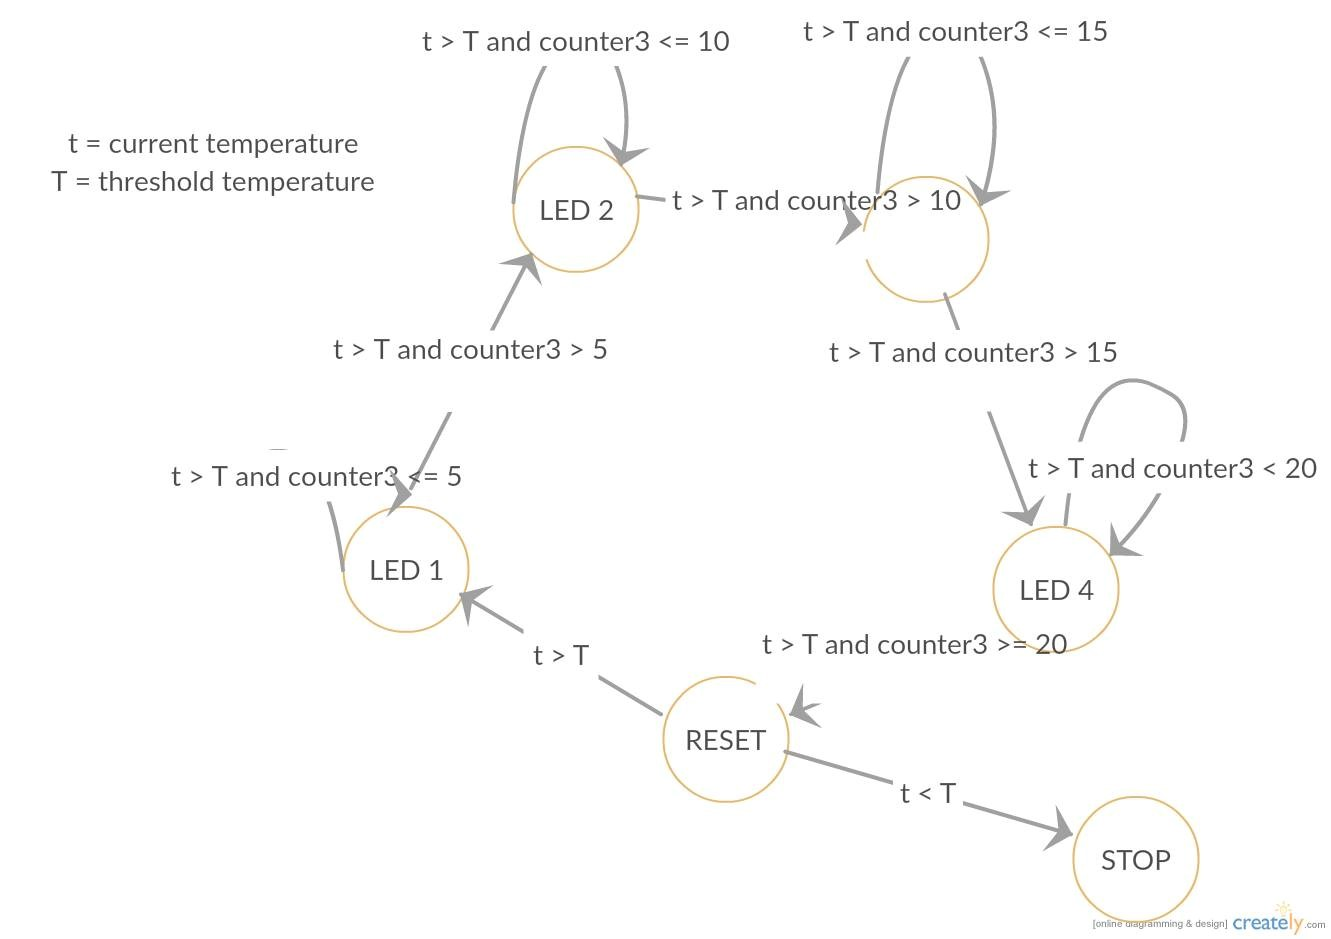
\includegraphics[width=11cm]{fig_1.jpg}
\caption{\small \sl State Diagram describing logic flow for 7-Segment display.}  
\end{figure}

\section{Testing and Observations}
After implementation was complete, the complete circuit was tested and observations were made that helped determine whether each part of the problem statement was implemented correctly and the goals achieved. The description of the tests and observations made, in the order they were tested, is provided below:

\begin{itemize}
\item \textbf{ADC and temperature sensor:} Before setting up the display, signal filtering and the overheating alarm, it was necessary to ensure that the ADC was set up correctly. For this it was simply noted whether we were able to print the correct voltage readings to the Keil terminal. Once that was complete, the temperature readings were obtained by using equation [2] and were similarly printed to the terminal. The calculated values of the temperature were between 28 and 30 degrees Celsius, thus validating the correct functionality of both the ADC and the sensor.
\item \textbf{Sampling frequency:} The frequency was set to 100Hz as per the project specifications and this was reflected in the Keil terminal output.
\item \textbf{Overheating alarm:} To test the overheating alarm, a hair blower was used to heat up the back of the Discovery board. The temperature rose steadily as expected. The threshold was set to be greater than 50 degrees Celsius and as soon as the temperature reading displayed 51 degrees Celsius, the LEDs lit up one by one and rotated as expected. The overheating alarm was, therefore, also fully functional.
\item \textbf{Temperature display:} Before testing the temperature display with the program, it was decided that the display should be tested independently. Due to issues with the original 7-sement display provided to us, a new display was chosen for use. After verifying that the new display lit up without any unusual behaviour, the circuit was built and then tested with the program. \\
\\Given the high sampling frequency, it was impossible to read the temperatures off the 7-segment display at first. To avoid this, the frequency at which the temperature in the 7-segment display changed was set to ~11.11Hz or once every 90ms. However, the sampling frequency was kept unchanged. To verify that this was working as intended, a separate print statement was issued to display the temperature only when it was also displayed on the 7-segment display. Both the display values and the terminal output values were compared and found to be the same up to 1 decimal points, thus verifying the functionality of the circuit.\\
\\One of the unresolved issues, however, was the slight flicker of the 7-segment display. Due to the rate at which each segment (one of four digits) changed, there appeared to be a slight flicker. While that was not very noticeable, a bigger side-effect was that the LED was quite dim. The brightness improved when we increased the display time period from 50ms to 90ms. Further tuning the display did not appear to be beneficial for the purposes of this project and so a different value was not chosen.
\item \textbf{Signal filtering:} To implement signal filtering and get rid of noisy data, the C implementation of the Lab 1 Kalman Filter was used. The voltage readings, which was the data containing the noise, was fed into the filter before being used to calculate the temperature. A sample test vector of various temperature readings was created and sent to the Kalman filter. To make use of this data, real-time temperature readings were calculated side by side and compared with. After getting satisfactory results, the parameters of the filter were changed.\\
\\In order to find the parameter that produced the best results, an open-source implementation of the Kalman Filter in Excel was used. This allowed the values of q and r to be varied while reflecting the change in a graph simultaneously. The rationale behind the choice of q and r values eventually used in the program was to find the best fit curve of the result. A preliminary choice of value 0.1 for both q and r provided the following curve:

\begin{figure}[!ht]
\centering 
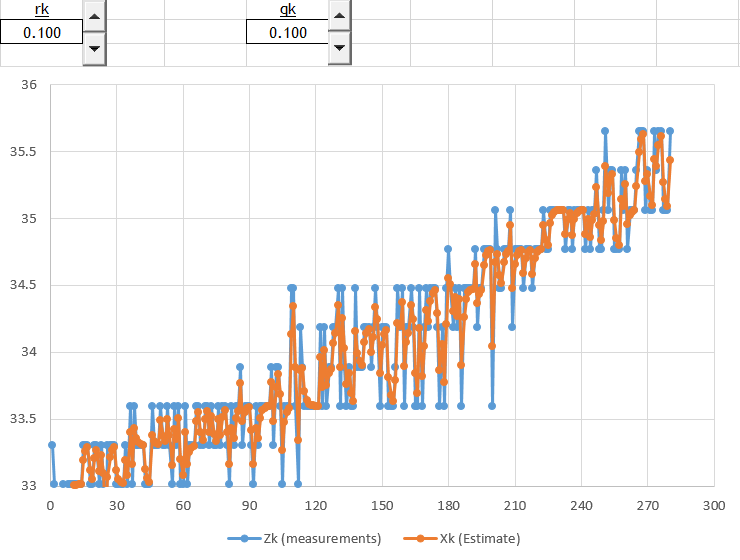
\includegraphics[width=7.5cm]{fig_2.png}
\caption{\small \sl Result of Kalman Filter with q=0.1 and r=0.1.}  
\end{figure}
\newpage

While these values allowed the estimate follow the actual measurements closely, it was not desirable to have such variance in the results. Therefore, the value of q was lowered and the value of r was increased. The resulting graph is given below:

\begin{figure}[!ht]
\centering 
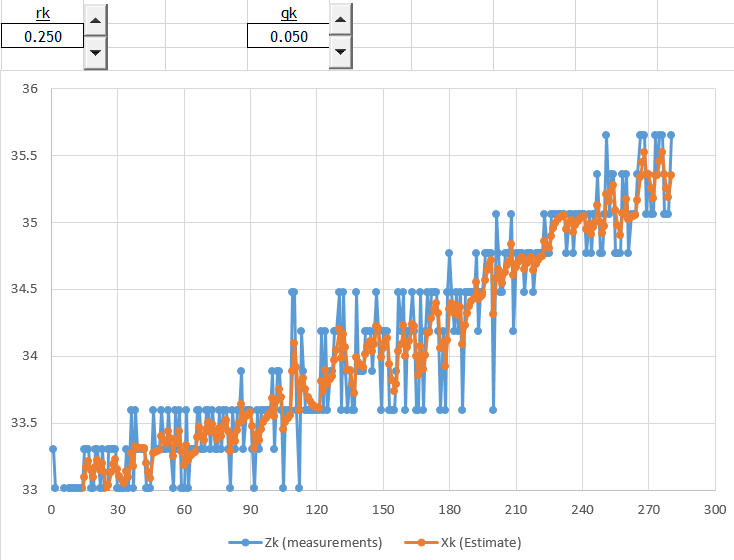
\includegraphics[width=7.5cm]{fig_3.png}
\caption{\small \sl Result of Kalman Filter with q=0.05 and r=0.250.}  
\end{figure}

This graph was a more accurate representation of what the aim was and after a lot of tinkering with different values, gave the best fit curve for the results. The final values for q and r were 0.014 and 0.550 respectively. Further change to these values would compromise the response time and was therefore avoided. The final graph that was obtained with the values is shown below:\\
\begin{figure}[!ht]
\centering 
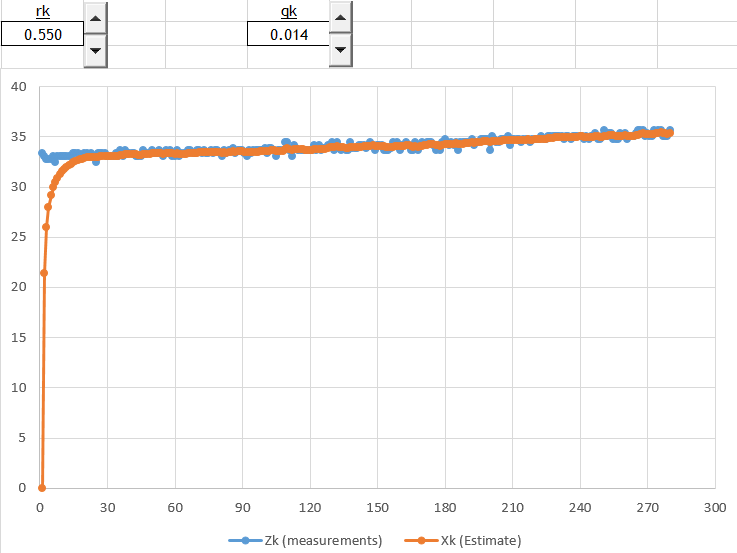
\includegraphics[width=7.5cm]{fig_4.png}
\caption{\small \sl Final output of Kalman Filter with q=0.014 and r=0.550.}  
\end{figure}

\newpage
A closer look showed the following graph:
\begin{figure}[!ht]
\centering 
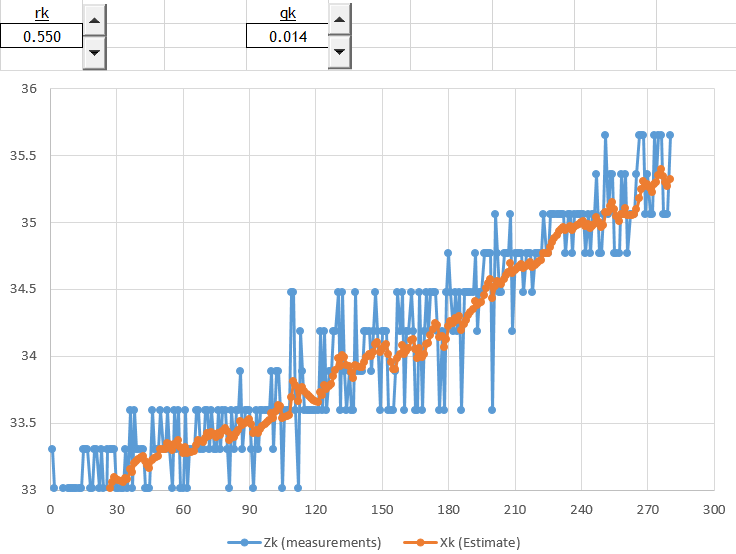
\includegraphics[width=7.5cm]{fig_5.png}
\caption{\small \sl Closer look at the result of Kalman Filter with q=0.014 and r=0.550.}  
\end{figure}

\end{itemize}

\section{Conclusion}
This experiment demonstrated the use of onboard sensors on the STM32F4 Discovery board and the use of ADCs to make use of raw data to obtain useful information such as temperature readings of the processor. Using the equation provided in a previous section, the temperature was calculated accurately and then displayed on the 7-segment display. The signal filtering was implemented in a way that suited the objective of this experiment. More specifically, the Kalman filter worked as intended and the temperature results were very close to the desired level of accuracy. The overheating alarm set off at temperatures over 50 degrees Celsius and switched off as soon as it fell below, as expected. 
\newpage

\section{Appendix}
\begin{itemize}
\item Kalman Filter Code in Python:\\
\\class KalmanFilter(object):\\
    \tabto{0.6cm}q;      // process noise covariance\\
    \tabto{0.6cm}r;      // measurement noise covariance\\
    \tabto{0.6cm}x;      // value\\
    \tabto{0.6cm}p;      // estimation error covariance\\
    \tabto{0.6cm}k;      // kalman gain\\

Reset():\\
    \tabto{0.6cm}q.value = q;\\
    \tabto{0.6cm}r.value = r;\\
    \tabto{0.6cm}x.value = x;\\
    \tabto{0.6cm}p.value = p;\\
    \tabto{0.6cm}k.value = k;\\
    
Kalmanfilter\_C():\\
    \tabto{0.6cm}p.value = p.value + q.value;\\
    \tabto{0.6cm}k.value = p.value / (p.value + r.value);\\
    \tabto{0.6cm}x.value = x.value + k.value * (noisy-measurement - x.value);\\
    \tabto{0.6cm}p.value = (1 - k.value) * p.value;\\

\item Code to extract individual digits from a decimal value:\\
\\ // sample is originally double valued in 1 decimal place\\
sample2 = sample * 10;\\
        
// set up loop counter\\
i = 0;\\                          

// at i = 0: store[i] contains the first decimal\\
// at i = 1: store[i] contains the least significant digit (prior to decimal)\\
while(i \textless \space 2)\{\\                   
    \tabto{0.6cm}store[i] = sample2 \% 10;\\   
    \tabto{0.6cm}sample2 /= 10;\\              
    \tabto{0.6cm}i++;\\
\}\\

// at i = 2: store[i] contains the most significant digit\\
store[2] = sample / 10;\\ 

\end{itemize}


























\end{document}